\section{Presentazione degli obiettivi}
Il nostro progetto per il corso di Reti di Calcolatori si è concentrato sullo sviluppo
di una applicazione di messaggistica per reti locali (LAN).
Si è progettato il programma in modo tale da
sfruttare il protocollo UDP per lo scambio dei messaggi, i quali si ipotizzano essere criptati tramite
crittografia asimmetrica con chiave pubblica/privata. Per di più, l'applicazione
è stata pensata per essere in grado di inviare anche allegati (che definiamo, a questo proposito,
come file generici quali immagini, audio, etc), anch'essi criptati.
Il programma, teoricamente, deve essere in grado di identificare tutti gli utenti connessi
alla LAN, così da rendere possibile scegliere con quale utente si desidera chattare,
similmente a quanto avviene con applicazioni note quali Skype o Telegram Desktop.
Inoltre deve godere di un'interfaccia grafica intuitiva per semplificare
le operazioni.

\section{Progetti a confronto}
L'idea della chat non è di certo innovativa. Ne esistono di molti tipi da diversi anni e
ognuna di loro ha manifestato il proprio momento di gloria, per poi abbandonare i riflettori
e dirigere gli utenti verso applicazioni più nuove e immediate.

Nell'ambito dei progetti realizzati in passato per il corso di Reti di Calcolatori,
in particolare, nel 2006 uno studente ha proposto un servizio di messaggistica su
connessione cifrata con SSL ad architettura p2p, non realizzando tuttavia tutte le premesse
e abbandonando quindi l'implementazione della cifratura con SSL e, di conseguenza,
la gestione dei certificati. Questo lavoro era stato svolto sfruttando la libreria Axis
di Apache Foundation.

Nel 2014 altri due studenti hanno realizzato una chat prevedendo un'unità centrale che
potesse immagazzinare i dati strettamente necessari sugli utenti, senza quindi affidare dati
ridondanti a tutti i client. Il loro obiettivo era quello di creare un servizio che fosse
a metà fra le chat peer to peer e le chat centralizzate.

\newpage
\section{Sviluppo degli Obiettivi}
Quasi tutte le parti poste nella Presentazione degli Obiettivi sono state correttamente
sviluppate e implementate. La chat realizzata possiede una GUI per l'interazione
con l'utente avente il seguente aspetto:
\begin{figure}[h]
\centering
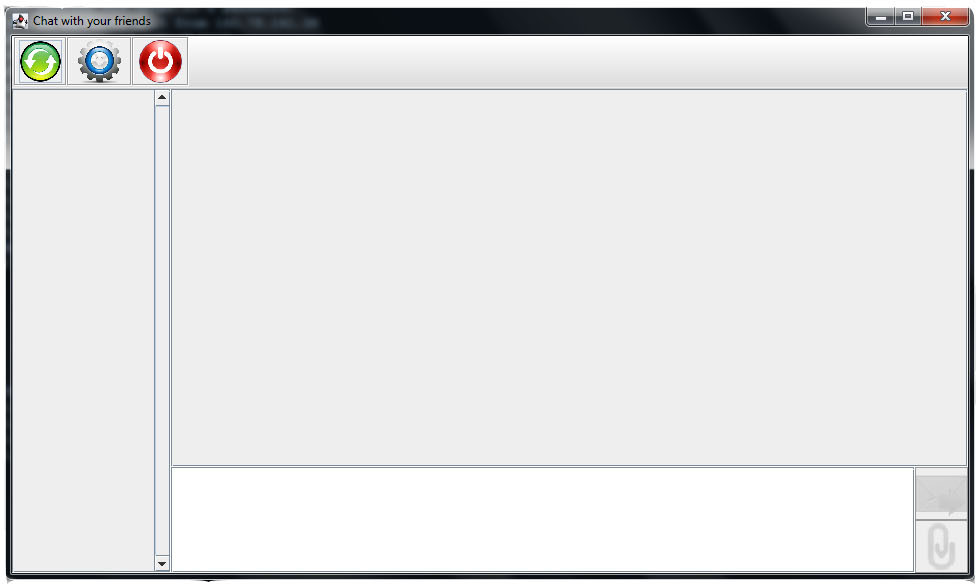
\includegraphics[scale=0.4]{gui1.jpg}
\caption{GUI principale\label{fig:gui}}
\end{figure}

Il riquadro in basso permette la scrittura di testo.
I due tasti laterali ad esso affiancati
consentono invece di inviare messaggi (criptati) o allegati (non criptati).
In alto sono presenti tre bottoni:
di essi, quello più a sinistra consente di scandire la rete per la ricerca di eventuali 
utenti che, in questo momento, stanno utilizzando la chat, tali utenti vengono salvati
in una lista di utenti conosciuti.
La scansione viene in ogni caso eseguita in automatico all'avvio del programma
e ripetuta periodicamente durante la sua esecuzione per aggiornare la suddetta lista.
Quando un utente viene trovato, nel riquadro a sinistra 
dell'applicazione viene inserito un pulsante con il suo nickname.
Cliccandoci sopra, diventa possibile chattare con lui e inviargli messaggi.
Il bottone al centro, invece, apre un'altra piccola finestra.

\begin{figure}[t]
\centering

\includegraphics[scale=0.3]{settings.png}
\caption{Pannello delle impostazioni\label{fig:settings}}
\end{figure}
Questa finestra gestisce le impostazioni e da qui l'utente può regolare:
\begin{itemize}
	\item ogni quanti secondi far eseguire la scansione della rete;
	\item ogni quante scansioni svuotare completamente l'insieme degli host conosciuti 
	in modo da non conservare inutilmente host non più presenti nella LAN o che abbiano
	chiuso l'applicazione;
	\item cambiare il suono di notifica che verrà riprodotto all'arrivo di un messaggio.
\end{itemize}
I pulsante più a destra invece consente di chiudere l'applicazione. Prima della
chiusura verrà mostrato un messaggio di conferma per chiedere all'utente se vuole davvero terminare
l'applicazione. Prima di essere chiuso, il programma manda a tutti gli host conosciuti
un messaggio speciale \emph{\#\#DOWN\#\#} in modo che gli altri host sulla LAN sappiano che si
sta disconnettendo e lo tolgano subito dalla lista degli host conosciuti.
All'avvio del programma si cerca il file di configurazione e si cerca di
leggere il nome utente e le impostazioni. In caso non venga trovato il file o il nome utente
non sia presente (è il primo accesso fatto dall'utente) compare una schermata di login:
\begin{figure}[h]
\centering
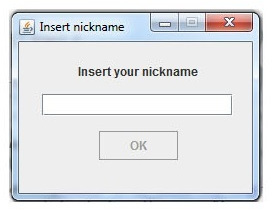
\includegraphics[scale=0.5]{login1.jpg}
\caption{Finestra di Login\label{fig:login}}
\end{figure}

In questa scheda l'utente crea il proprio account, scegliendo un nickname da usare in chat.
Una volta digitato il nickname, il tasto di conferma diventa abilitato e premendolo si effettua
il login, consentendo finalmente l'uso vero e proprio dell'applicazione.
Viene poi controllata la presenza della coppia di chiavi e nel caso non siano presenti vengono create.
\\

In questa relazione, analizzeremo a grandi linee la codifica proposta e l'implementazione
delle varie classi, con particolare enfasi sul ruolo giocato da ognuna di esse.
Mostreremo, poi, i risultati ottenuti e, infine,
il funzionamento dell'intero programma qui presentato,
esponendo anche i test fatti in corso d'opera
in locale e sulla Virtual Private Network di ateneo.
Il lavoro svolto sarà, quindi, accompagnato dalle dovute conclusioni e
da un commento sui possibili sviluppi futuri.